\prefacesection{Assignment}

\section*{Design of Network}
Initially, the design of the network will consist of two input nodes for the two values contained in the training dataset. The learning rate will be set to 0.01 because it said that is a good rate to begin training at (https://www.youtube.com/watch?v=jWT-AX9677k). This rate will be reduced after each number of runs. On the output layer, only one output node will be made to output the predicted value.
The network shall also contain one hidden layer. This will consist of two nodes but will be increased incrementally to evaluate the optimal number.
The goal of this network is see what the optimum network topology is to reduce the error in the shortest amount of time. 

\begin{figure}[ht]
	\begin{center}
		\advance\leftskip-3cm
		\advance\rightskip-3cm
		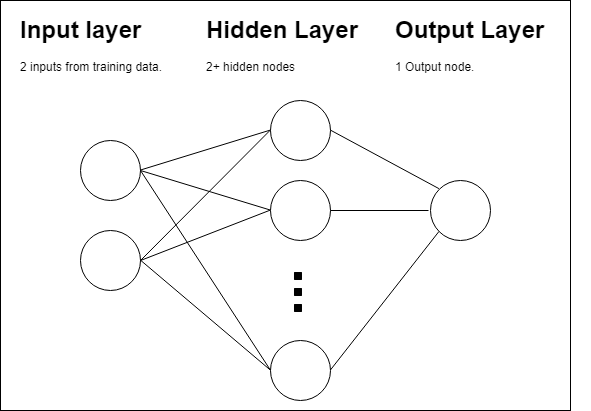
\includegraphics[keepaspectratio=true,scale=0.6]{__resources/networkarch.png}
		\caption{Architecture of neural network}
		\label{member2}
	\end{center}
\end{figure}

\newpage
\section*{Network Training}
In this section we shall train the network. Each score declared in the tables are an average score over ten runs for each parameter. This process was done incrementally by first deciding a number of epochs, this is followed by a number of hidden layer nodes. And lastly, decreasing the learning rate from 0.01 to 0.0001.

\subsection*{1000 Epochs}
A good starting off point to train the network began with a thousand epochs. Initially the network was trained with 2 hidden layer nodes for 1000 epochs. The cost, error and time are measured and the average over ten runs is calculated.
\newpage
\subsubsection*{2 Hidden Layer Nodes}
In the table 1 it can be seen that although the training time is low, the error rate never met the satisfactory rate 0.01, and the cost is relatively high. Therefore, it can be noted that is not a desirable model.

 \begin{longtable}{|>{\raggedright\arraybackslash}p{3cm}|c|c|c|c|}
	\hline 
	Learning rate & Cost & Error & Time \\ 
	\hline 
	0.01 & 51.992 & 0.14 & 0.932 \\ 
	\hline 
	0.001 & 58.2 & 0.1916 & 1.006 \\ 
	\hline 
	0.0001 & 119.40 & 0.504 & 0.846 \\ 
	\hline 
	\caption{Two Hidden Layer Nodes for 1000 Epochs}
 \end{longtable}


\subsubsection*{3 Hidden Layer Nodes}
The three node model performed significantly better than the previous, with a low error score of 0.0098 on the learning rate 0.01, so this model can be taken into consideration saving and evaluation. However, the other scores did not meet the tolerable error score as the learning rate was decreased, as seen in Table 2.\\
 \begin{longtable}{|>{\raggedright\arraybackslash}p{3cm}|c|c|c|c|}
	\hline 
	Learning rate & Cost & Error & Time \\ 
	\hline 
	0.01 & 1.34 & 0.0098 & 0.72 \\ 
	\hline 
	0.001 & 17.83 & 0.116 & 0.89 \\ 
	\hline 
	0.0001 & 119.47 & 0.495 & 0.874  \\ 
	\hline 
	\caption{Three Hidden Layer Nodes for 1000 Epochs}
\end{longtable}

\subsection*{2000 Epochs}
Following a successful attempt with the previous model, further experimentation was done by increasing the number of epochs the network will be trained with.
\subsubsection*{2 Hidden Layer Nodes}
Firstly, the network is reduced back to 2 hidden layer nodes and the average scores of the cost, error and elapse time are calculated. As seen in Table 3, no improvement was made to the model as the cost, error and training time were all increased.

 \begin{longtable}{|>{\raggedright\arraybackslash}p{3cm}|c|c|c|c|}
	\hline 
	Learning rate & Cost & Error & Time \\ 
	\hline 
	0.01 & 50.77 & 0.147 & 1.606 \\ 
	\hline 
	0.001 & 51.985 & 0.123 & 1.606 \\ 
	\hline 
	0.0001 & 115.24 & 0.49 & 1.62  \\ 
	\hline 
	\caption{Two Hidden Layer Nodes for 2000 Epochs}
\end{longtable}


\subsubsection*{3 Hidden Layer Nodes}
Secondly, an extra node was added to the model. It can be noted from Table 4 that a significant improvement was made to the model by adding an extra node to the hidden layer. The cost was reduced to 0.658 and error to 0.0053 when the learning rate was set to 0.01. 
 \begin{longtable}{|>{\raggedright\arraybackslash}p{3cm}|c|c|c|c|}
	\hline 
	Learning rate & Cost & Error & Time \\ 
	\hline 
	0.01 & 0.658 & 0.0053 & 1.94 \\ 
	\hline 
	0.001 & 8.72 & 0.054 & 1.81 \\ 
	\hline 
	0.0001 & 117.19 & 0.489 & 1.66  \\ 
	\hline 
	\caption{Three Hidden Layer Nodes for 2000 Epochs}
\end{longtable}


From these figures it is evident that the 2 node model that was trained for 1000 epochs and the 3 node model that was trained for 2000 epochs performed the best. Although the training time is shorter with 2 node network, the latter has a better accuracy. It should also be taken into consideration that there is only an average of 1.22 second training time difference, which is not a high cost to pay. Therefore, the model with 3 hidden layer nodes that, trained for 2000 epochs, and the learning rate set to 0.01 shall be used for evaluation.

\section*{Network Evaluation}
Upon inspection of the trained models results, the model was again trained with the optimal parameters specified and saved to disk, but upon evaluating the model with new data, the model did not perform as well as it did when training.
An average overall error of 0.02775318, over 10 runs, was the result of using this model. Therefore, further training was implemented. In order to reduce the error, the number of nodes and epochs were increased incrementally. These numbers are average results over 10 runs from the evaluation scripts in respect to the newly trained models. All models were trained with the 0.01 learning rate as it proved to provide the best results. See Table 5 for results.

 \begin{longtable}{|>{}p{4cm}|c|c|}
	\hline 
	Number of Epochs & Nodes & Average Error\\ 
	\hline 
	3000 & 3 & 0.02332\\ 
	\hline 
	3000 & 4 & 0.0224\\ 
	\hline 
	3000 & 5 & 0.0184\\ 
	\hline
	3000 & 6 & 0.0128\\ 
	\hline	
	3000 & 7 & 0.0175\\ 
	\hline
	3000 & 8 & 0.0125\\ 
	\hline 
	\hline
	4000 & 3 & 0.0256\\ 
	\hline	
	4000 & 4 & 0.0139\\ 
	\hline	
	4000 & 5 & 0.0143\\ 
	\hline	
 	4000 & 6 & 0.0118\\ 
	\hline	
 	4000 & 7 & 0.0121\\ 
	\hline
 	4000 & 8 & 0.0118\\ 
	\hline
	\hline
	5000 & 3 & 0.0184\\ 
	\hline	
	5000 & 4 & 0.0146\\ 
	\hline	
	5000 & 5 & 0.0145\\ 
	\hline	
	5000 & 6 & 0.0115\\ 
	\hline	
	5000 & 7 & 0.0105\\ 
	\hline
	\textbf{5000} &\textbf{8 }& \textbf{0.0093}\\
	\hline 
	\caption{Incremental Experimentation with Parameters}
\end{longtable}

As seen from this iterative process in the table above, the most optimal model for evaluation required 8 hidden layer nodes and to be trained for 5000 epochs in order to result in a error below 0.01.


\section*{Conclusion}
In conclusion, the model received two inputs, one hidden layer and one output. The network was trained using 500 examples in the training dataset. The model performed well during training with 3 hidden layers nodes, but failed to reach the minimum tolerable error when given new data. Therefore, further experimentation was conducted in order to find the optimal number of training epochs, learning rate and nodes that were required in order to reach an error below 0.01 in the evaluation phase. The project was successful in implementation, with an average evaluation error of 0.00093.
